\documentclass{article}
\usepackage{mathtools}
\usepackage{amssymb}
\usepackage{graphicx}

\usepackage{natbib}

\usepackage[hidelinks]{hyperref}

\usepackage{wrapfig}

\usepackage{url}

% For an article, maybe organise as follows :
%   Method
%       ROI
%       Computational Graphs
%   Experiments
%       CNN ROI
%       Transformer ROI vs attn head (for circuit discovery and ... ? Maybe sort by attribution on tasks as in CNN ROI and ablate like this, then show that ROI better than attn head ?) Are identified important ROIs "interpretable" ? Very simple experiment : show overlap between ROI and attn head (concat head dicts).
%       Compare our algorithm with marks (edge attribution different, node ablation vs edge ablation)
%       Compare our algo with AtP
%       ...


% TODO : schema d'un graph de calcul séparé par module -> contract ROI vs contract attn head
%   another to show that feature in single module are not effectively connected to one another so we regroup them by functionnality / to show that for the whole model is too big but for one module is ok

\usepackage[capitalize,nameinlink]{cleveref}

\usepackage{subcaption}

\newcommand{\R}{\mathbb{R}}
\newcommand{\Q}{\mathbb{Q}}
\newcommand{\N}{\mathbb{N}}

\widowpenalty=10000
\clubpenalty=10000

\usepackage[a4paper, margin=1.in]{geometry}

\begin{document}

\title{Emerging Structures in Computational Graphs of Neural Networks}
\author{
    Grégoire DHIMOÏLA \\
    ENS Paris-Saclay \\
    \texttt{gregoire.dhimoila@ens-paris-saclay.fr}
}
\date{March - August 2024}
\maketitle

\newpage
\begin{abstract}

While neural networks form the basis of modern machine learning, their inner workings are still far from well understood. To comprehend neural networks' (NN) behaviors and ensure their safe and fair application, a key direction is to measure and interpret their internal mechanisms. The field of mechanistic interpretability aims to explain these internal mechanisms. One of its main framework is \emph{circuit discovery}, which attempts to find and interpret subsets of computational nodes responsible for certain tasks or functionalities.

Mechanistic analyses of NNs commonly involve neurons, which are often polysemantic and hard to interpret, or to disentangle them into features. They are fine-grained units of analysis in that they provide a high level of information and detail. In this work, we introduce regions of interest (ROIs) as sets of functionally similar features for low granularity studies of computational graphs. We show the functional relevance of these ROIs.

We then propose an algorithm that finds computational graphs through causal relationships between nodes. This algorithm is general in that it can accommodate  nodes of arbitrary granularity, from features to attention heads or ROIs. We systematically compare desired functional and structural properties of these graphs.
\end{abstract}

\newpage
\tableofcontents

\newpage
\section{Introduction}

Developing tools to study the internal mechanisms of neural networks~(NN) is key in the understanding of their internal representations, world models and what algorithms they can implement. These insights help identify and prevent potential biases \citep{marks2024sparseCircuits} and lead to the design of interventions to predictably steer the model's behavior \citep{turner2024activationSteering,panickssery2024steeringllama2contrastive}.

The field of \textit{mechanistic interpretability} (MI) aims at explaining these internal mechanisms. This usually results either in the attribution of some function or behavior to a specific computational units \citep{mallen2024elicitinglatentknowledgequirky, marks2023geometrytruthemergentlinear, lu2019checking} or to a subgraph of the network formed by these units \citep{conmy2023automatedACDCCircuits, merullo2024talking}. We see in \cref{sec:parallels} that both of these approaches have historical equivalents in the field of neurosciences.\\

The current MI framework relies heavily on sparse coding to learn disentangled and more interpretable \textit{features}, encoding concepts and generating representations. Features in later layers can be viewed as functions of earlier features, and the model can then be thought of as a large composition of these simple functions. When conducting mechanistic analyses in language model, it is common practice to use these features as units of analysis for high-level - fine-grained - information \citep{marks2024sparseCircuits}, or to use attention heads for coarser, lower-level insights \citep{conmy2023automatedACDCCircuits,syed2023attributionCircuits}.

\textit{Circuit discovery} in MI aims to find computational subgraphs responsible for some selected task or behavior \citep{conmy2023automatedACDCCircuits, syed2023attributionCircuits, oneill2024sparse, he2024dictionaryCircuits}. They mostly focus on finding which nodes best explain a behavior and providing manual interpretations of them \citep{marks2024sparseCircuits, conmy2023automatedACDCCircuits} leading to denser graphs (see \cref{sec:node_edge_ablation}). This can be fine for task specific studies where the number of nodes involved in the task is significantly smaller than the total number of nodes.

However, if we want to do more general studies of the computations of the model, these approaches would basically leave the computational graph unaltered as most nodes are likely to be relevant in at least one context. For this reason, we believe that circuit discovery studies should evaluate actual subgraphs through edge ablation rather than focusing on the subsets of nodes fully connected through node ablation (\cref{sec:node_edge_ablation}).

The purpose of this study is to construct faithful and sparse computational graphs and investigate their structures.\\

%The original plan for this internship was as follow. First, define a way to get a computational graph for the general computation of a neural network. Then, study the properties of these graphs as well as their structures. Interpret these structures and label each node with a simple functions. Do this across training step and compare the different graphs to study the evolution of these structures, and do it across model sizes to study their universality. This proved to be quite ambitious and we primarily focused on how to build an interesting graph and how to study its structures.\\

This work is organised as follows. In \cref{sec:meta}, we give general comments on the internship. In \cref{sec:background}, we provide some background on notions from neurosciences\footnote{Due to the large overlap between the means of study of brain networks (\cref{sec:brain_networks}) and artificial neural networks (\cref{sec:interpretability}), we try to use terminology from the field of neurosciences wherever relevant.} (\cref{sec:brain_networks}), network sciences (\cref{sec:SBM}) and MI (\cref{sec:SAE,sec:interpretability}). These notions are the basis upon which we build our discussions and contributions. In \cref{sec:parallels}, we draw parallels between the way neurosciences and MI explain complex systems through the analysis of underlying networks or structures. Following sections contain our contributions.\\

\begin{wrapfigure}{r}{0.42\textwidth}
    \vspace{-4.em}
    \centering
    \includegraphics[width=0.4\textwidth]{images/intro/ROI_illustration.pdf}
    \caption{Illustration of ROIs in a the feature extractor of a simple CNN. Features are sorted by ROI. ROI are sorted by most activating class.}
    \label{fig:ROI_illustration}
\end{wrapfigure}

We introduce in \cref{sec:ROI} a novel algorithm to partition features by functional equivalence. We call the resulting class \emph{regions of interest} (ROIs). ROIs give coarse units of analysis for any further mechanistic study of the model. Typically, while circuit discovery often uses attention heads in transformers as low granularity\footnote{Granularity refers to the level of detail and information captured by nodes} nodes, this approach may be suboptimal as these units are often polysemantic and hard to interpret outside of specific contexts. Moreover, there is no equivalent in MLP layers. We provide a set of experiments to validate the relevance of these groups. We did not yet compare the use of ROIs and attention heads in mechanistic studies, which is left for future~work.\\

\begin{wrapfigure}{l}{0.43\textwidth}
    \vspace{-4.em}
    \centering
    \includegraphics[width=0.48\textwidth]{images/intro/circuit_illustration.pdf}
    \caption{Illustration of a computational graph for a mixture of three different language tasks.}
    \label{fig:circuit_illustration}
\end{wrapfigure}
~\\
\paragraph{}\cref{sec:computational_graphs} describes a general class of algorithms using attribution to construct a computational graph. It can accommodate several levels of granularity. For example, when working with fine-grained features as nodes, the resulting algorithm is similar to that introduced by \citet{marks2024sparseCircuits}, though some details for edge attribution are different. When using coarser nodes like attention heads, it simplifies to the algorithm from \citet{syed2023attributionCircuits} with a different attribution method - integrated gradients instead of raw gradients (see \cref{sec:attribution}). In this section, we also provide some preliminary results on the properties of these graphs.
~\\
\paragraph{Contribution.} We propose to study emerging structures in computational graphs to improve and automate MI, using both \textit{functional} and \textit{causal}\footnote{This would be referred to as \textit{effective} connectivity in neuroscience} relationships between nodes.
\begin{itemize}
    \item We define new low granularity nodes for the study of neural networks as groups of \textit{functionally} similar fine-grained nodes\footnote{Fine-grained nodes can be anything from canonical dimensions - also known as neurons - to sparse features through any change of basis relevant to the model internal geomerty.} (\cref{sec:ROI}) as defined by \textit{Stochastic Blockmodels} (SBM) (\cref{sec:SBM}). We call these \emph{regions of interest} (ROIs).
    \item We establish the relevance of these ROIs through interventions and predictable behavioral changes in the model (\cref{sec:ROI_exp}) and show that ROIs given by SBMs are functionally more relevant than those given by community detection algorithms commonly used in the literature (see \citet{lu2019checking, filan2021clusterability, bushnaq2024using}). % FUTURE WORK (very close !) ROI graph vs attention heads graphs, often used in the literature as low granularity nodes as well as easier interpretability
    \item We define a novel algorithm to construct computational graphs in neural networks that can incorporate several levels of abstraction (\cref{sec:effective_connectivity}) along with methods to study these graphs.
    %\item[FUTURE WORK] We establish the superiority of Stochastic Blockmodels over more traditional community detection algorithms in studying the structure of these graphs.
    \item We show the relevance of these methods by demonstrating the functional equivalence between the original model and the one induced by our computational graph (\cref{sec:computational_graphs_exp}), as well as intervening on this graph with predictable effects on the resulting model's behavior. Our results outperform those of previous research.
    %\item[future work] We show that restraining a model to its elicited computational graph can naturally remove sleeper agents without intervention and that interventions on this graph can further remove unwanted behaviors (\cref{sec:___}).
\end{itemize}

In \cref{sec:future} we discuss shortcomings of the current study and directions for future work.

\section{Meta Information}
\label{sec:meta}

This section provides an overview of the meta aspects of my internship, including supervision, team environment, key events and a rough timeline.

A publication relative to the work done during this internship is currently planned.

\subsection{Supervision and Environment}

During my internship, I received substantial support from my supervisor - Prof. Holger Dell - who was consistently available and engaged. We had discussions basically on a daily basis, allowing for continuous feedback and guidance. He organized meetings with various teams, enabling me to present my work, receive constructive feedback, and explore potential collaborations.

Overall, the lab was welcoming and open to discussion throughout my internship. I was able to gain understanding from the inside of how a lab operates on both teaching and research aspects.

\subsection{Events}

Throughout the internship, I participated in a range of events. These included seminars and meetings with both my team and other teams on a regular basis. These gatherings provided opportunities to present our work, brainstorm new ideas, and explore potential collaborations.

Noteworthy events included the HAAISS Summer School and the ICML Conference both in July. At the summer school I was able to meet a substantial amount of the MI community. At ICML I presented some of my work as part of a workshop, which was my first experience in this kind of events.

\subsection{Timeline}

\begin{itemize}
    \item In depth exploration of the field of MI, preliminary work on several potentially interesting directions\dotfill1~month
    \item Focus on one promising direction: use attribution methods on feature compositions to construct a graph of dependencies\dotfill1 month
    \item First experiments and results\dotfill1 month
    \item Discovery and exploration of the SBM literature\dotfill2 weeks
    \item HAAISS Summer School\dotfill1 week
    \item ICML conference\dotfill1 week
    \item Report writing and further experiments\dotfill1 month
\end{itemize}

\section{Background}
\label{sec:background}

This section gives some background on notions from neurosciences (\cref{sec:brain_networks}), network sciences (\cref{sec:SBM}) and mechanistic interpretability (\cref{sec:SAE,sec:interpretability}). These notions are the fundations upon which we build our work.

\subsection{Notations}
\label{sec:Notations}

We regroup here some notations that may come handy later on. In particular, notations relative to sparse autoencoders will be introduced again and explained in \cref{sec:SAE}.

We will denote by $\mathcal{M}$ a neural network model, and by $m$ its \textit{modules} - MLP layers for multi-layer perceptrons (MLP), transformer blocks, attention layers or attention heads for transformers, convolutional layers for convolutional neural networks (CNNs).

For transformers, the dimension of the residual stream will be denoted by $d_{\mathrm{model}}$. When $\mathcal{M}$ denotes a model with an arbitrary architecture, $d_{\mathrm{model}}$ will be the dimension of the input and we call $d_{m}$ the dimension of the output of module $m$ in general. The output of module $m$ on input $x$ will be denoted by $x^m \in \R^{d_m}$.

For all modules $m$ let
\begin{align*}
&E_m : \R^{d_{m}} \rightarrow \R^{d_{\mathrm{dict}}}\\
&D_m : \R^{d_{\mathrm{dict}}} \rightarrow \R^{d_{m}}
\end{align*}
be an encoder and decoder pair, with $f^m = E_m(x^m)$. These can be arbitrary autoencoders, from a linear change of basis to a gated SAE - see \cref{sec:SAE}. Each canonical dimension $i < d_{\mathrm{dict}}$ of the dictionary will be called a feature, its associated feature vector $b_i$ in the weights of the dictionary $D_m$ is supposed to be unitary, and the magnitude $\alpha_i = f^m_i$ of the activation of this feature on any input will be called the feature's activation. We will often identify $b_i$ and $\alpha_i$ under the notation $f_i$ or simply $f$, for feature.

Scalar functions depending on the evaluation of $x$ by $\mathcal{M}$ will be denoted by $\lambda$. It can be a metric function on the output of the model, or any scalar function depending on its internal activations.

\subsection{Brain Networks}
\label{sec:brain_networks}

The field of neurosciences has been trying to understand the brain by explaining the function of each of its parts. There are two main paradigms when trying to explain the function of the brain: \textit{functional segregation} and \textit{functional integration} of brain regions \citep{tononi1994measure, sporns2013network, pavlovic2015generalised}. The former, which historically appeared first, assumes that the brain is divided into many parts, each specialising in various functions by engaging in local processes, while the latter assumes that the brain is a complex network of neuronal elements whose connections facilitate different functional processes. \textit{Functional integration} has been shown to be more successful in explaining higher cognitive processes like visual recognition, social cognition or emotions \citep{van2013network}.

When it comes to building a brain network, three major classes of connectivity can be distinguished: \textit{structural}, \textit{functional} and \textit{effective} connectivity \citep{hagmann2007mapping, friston2011functional}. Structural connectivity refers to the anatomical connections between brain regions. Functional connectivity measures temporal correlations between the activation of brain regions, the idea being that regions that share the same function, or work together in the emergence of more complex ones should be active at the same time. Effective connectivity measures causal relationships between brain regions through actual information flow.

\subsection{Block Models}
\label{sec:SBM}

Block Models \citep{daudin2008mixture, Peixoto_2019} are a class of generative models for graphs. For a graph with $n \in \N$ nodes, they assume that the nodes are partitioned into $B \leq n$ blocks and that the edge probabilities are summarised in a matrix $P \in \R^{B\times B}$ such that the probability of an edge $(i, j)$ with nodes assigned respectively to block $b_i$ and $b_j$ depends only on these blocks and is given by $P_{b_i, b_j}$. The adjacency matrix $A$ is then generated by sampling each entry $A_{ij}$ from a Bernoulli distribution with parameter $P_{b_i, b_j}$.

This is a generalisation in blocks of the Erdos-Renyi model, which corresponds to the case where $B = 1$. It can model a large variety of graph structures, some of which are presented in \Cref{fig:SBM_structures}.

\begin{figure}[h]
    \centering
    \begin{subfigure}{0.3\linewidth}
        \centering
        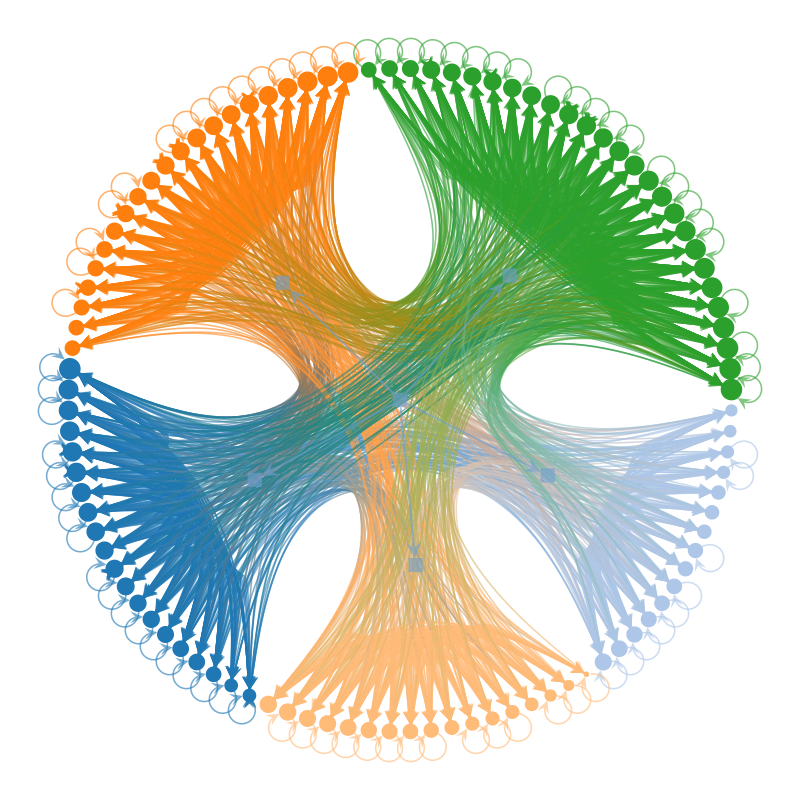
\includegraphics[width=\linewidth]{images/sbm/modular.png}
    \end{subfigure}
    \hfill
    \begin{subfigure}{0.3\linewidth}
        \centering
        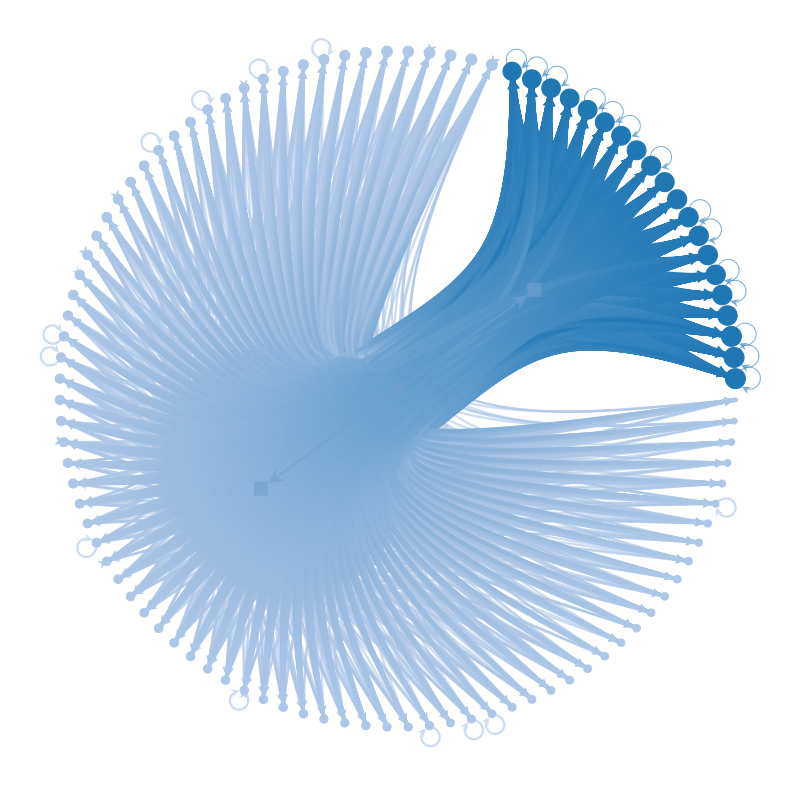
\includegraphics[width=\linewidth]{images/sbm/core_periphery.png}
    \end{subfigure}
    \hfill
    \begin{subfigure}{0.3\linewidth}
        \centering
        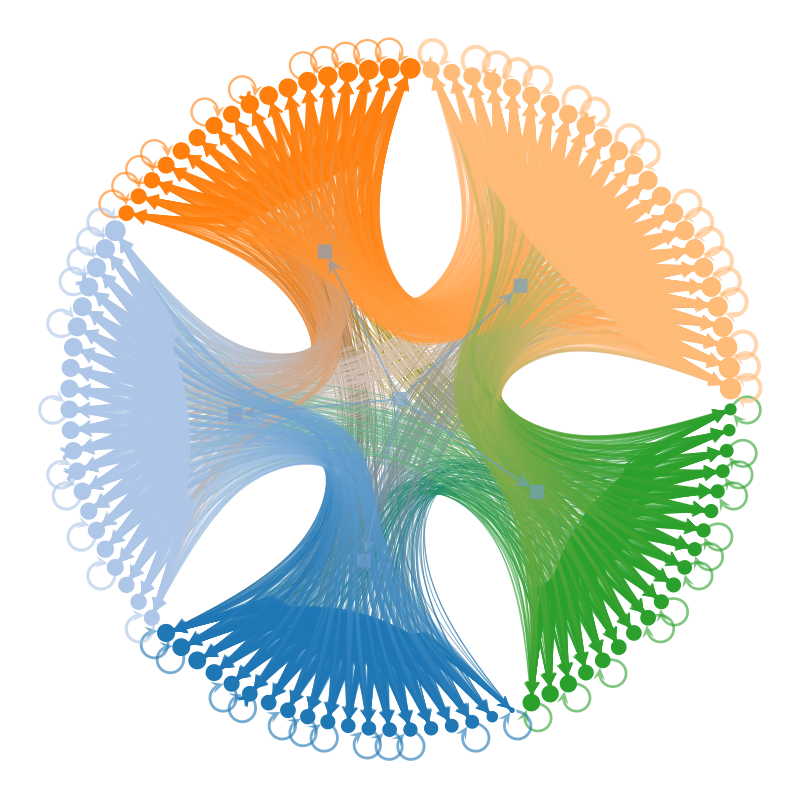
\includegraphics[width=\linewidth]{images/sbm/ordered.png}
    \end{subfigure}
    \vspace{1em}
    \begin{subfigure}{0.3\linewidth}
        \centering
        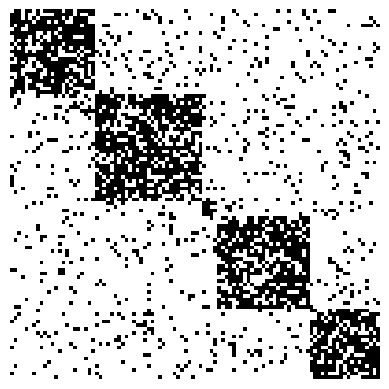
\includegraphics[width=\linewidth]{images/sbm/modular_adj.png}
        \caption{modular}
        \label{fig:modular_adj}
    \end{subfigure}
    \hfill
    \begin{subfigure}{0.3\linewidth}
        \centering
        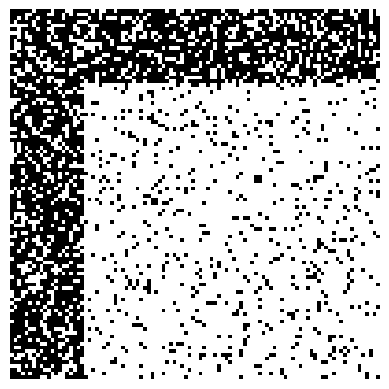
\includegraphics[width=\linewidth]{images/sbm/core_periphery_adj.png}
        \caption{core-periphery}
        \label{fig:core_adj}
    \end{subfigure}
    \hfill
    \begin{subfigure}{0.3\linewidth}
        \centering
        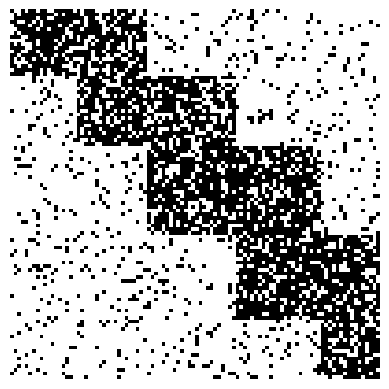
\includegraphics[width=\linewidth]{images/sbm/ordered_adj.png}
        \caption{ordered}
        \label{fig:ordered_adj}
    \end{subfigure}
    \caption{Examples of graphs with block structure recovered by a SBM. \emph{Top row}: contains visualisations of the graphs with nodes ordered and colored by block. The size of the arrow represent the number of edges between blocks. \emph{Bottom row}: shows the corresponding adjacency matrix.}
    \label{fig:SBM_structures}
\end{figure}

One can either use this framework to generate random graphs with a given structure, or to infer the underlying structure of a given graph. In the latter case, the goal is to find the block structure that maximises the likelihood of the observed graph. We will focus on the latter and fit Stochastic Block Models (SBMs) \citep{Peixoto_2019, lee2019review} to a given graph - in our case, it will be the computational graph of a neural network.\\

Community detection algorithms are commonly used in the fields of neurosciences \citep{chen2013inferring} and neural networks \citep{filan2021clusterability, bushnaq2024using} to try to find the underlying structure of complex networks and hopefully explain some mechanisms of the overall function of the model. However, these algorithms assume that nodes are arranged in communities - where nodes are densely connected within communities, but sparsely between communities - which restricts the possibilities on the discovered structures. Moreover, they are often prone to overfitting, where community structure is discovered even though it is merely an artefact of random fluctuations - see \citet{Peixoto_2019}.\\

SBMs allows us to relax these assumptions and find more general structures. Through the choice of clever prior distributions in Bayesian models \citep{Peixoto_2019}, they allow to avoid the pitfall of underfitting as well as overfitting statistical fluctuations in the data by finding blocks that do not account for statistically significant structures in the data that can't be explained by random fluctuations. Underfitting is mainly avoided through recursive block models to get the likelihood of some choice for the probabilities between blocks, which also enables the discovery of nested structures in the data. Efficient inference algorithms arise from the choice of these priors and bayesian frameworks, using Markov Chain Monte Carlo methods to find the block structure that maximises the likelihood of the observed graph.

SBMs were succesfully used in neurosciences \citep{pavlovic2015generalised, peixoto2018nonparametric} to identify established brain structures and advance the field as a whole. They were able to identify both functional segregation in modular parts of the network and functional integration in densely connected cores.

\subsection{Sparse Autoencoders}
\label{sec:SAE}

\paragraph{Linear Representation Hypothesis.} The linear representation hypothesis assumes that a model's latent space behaves mostly linearly, with high level concepts represented as disantangled directions in this space often called features. It also states that linear directions can be found using linear probes and that they can be used as steering vectors to predictably influence the model's behavior. Evidence of all these aspects can be found in \citet{park2023linear, NIPS2013_9aa42b31, pennington2014glove, nanda2023emergent, gurnee2024language, wang2024conceptSteering, turner2024activationSteering}.

\paragraph{Sparse coding.} This motivates the use of dictionary learning and sparse coding methods to find overcomplete bases able to sparsely represent the data at any point in the model. The hope here is that the learnt dictionary's feature vectors correspond to actual features used by the model. Formally, for some module $m$ we want a family $\{b_i \in \R^{d_{m}}\}_{i=0}^{d_{\mathrm{dict}}}$ such that, for all activations $x^m$, there is a set $\{\alpha_i \in \R\}_{i=0}^{d_{\mathrm{dict}}}$ mostly 0 such that $x = \sum_{i=0}^{d_{\mathrm{dict}}} \alpha_i b_i$. There are two dual problems here, one is to find such a family, the other is, given a family and a data point, to find the $\alpha_i$.

\paragraph{Notation.} In the rest of this work, these $b_i$ will be unit vectors called features, and both $b_i$ and its magnitude $\alpha_i$ will be identified under the notation $f_i$, as announced in \cref{sec:Notations}.

\paragraph{Autoencoders.} People usually train sparse autoencoders (SAE) ($E_m$, $D_m$) to solve both of these problems. The decoder $D_m$ serves as the dictionary, with its weight matrix containing the $b_i$ in column, while the encoder $E_m$ is the sparse coding function.

The majority of current research in transformer interpretability uses one layer MLPs \citep{cunningham2023sparse, gao2024scaling} trained to learn the identity function with an added sparsity loss. \citet{rajamanoharan2024improving} proposed an improvement to this method by adding a gated mechanism to the MLPs.

\citet{bushnaq2024using} introduced a change of basis called the \textit{Local Interaction Basis} (LIB) that can be viewed as a linear autoencoder capturing functionally important features, though the decomposition is not sparse. Any relevant change of basis found by future research can be similarly used as a linear autoencoder.%`FUTURE`

All of this work finds highly interpretable features, and is one direction in trying to find better geometric representations of model's latent space.

\subsection{Interpretability}
\label{sec:interpretability}

We provide here some background on previous interpretability work (\cref{sec:attribution,sec:circuit_discovery}), on some key implementation details (\cref{sec:node_edge_ablation}) and on current limitations of these methods.

\subsubsection{Attribution and explanations}
\label{sec:attribution}

In this section, we discuss classical attribution methods in neural networks. Attribution is the process of explaining a model's prediction by attributing it to some part of the input or intermediate feature. This is a very active field of research, and many methods have been proposed.

We begin with the most basic and popular methods. \citet{springenberg2015strivingGuidedBackprop} used gradient in vision models to highlight which pixels of an image best explain some output. Let $\lambda : x \in \R^{d_{\mathrm{model}}} \mapsto \lambda(x) \in \R$ be a scalar function on the model's computations - say the output value for a given class in a classifier - and $x \in \R^{d_{\mathrm{model}}}$ an input image of size $d_{\mathrm{model}}$.

$$ \mathrm{Attr}(x_i) = \frac{\partial \lambda(x)}{\partial x_i} $$

They show that even though results are satisfactory, the explanation is really noisy and imprecise. They introduce guided backprop, a variant that removes negative gradients in \emph{ReLU} - Rectified Linear Unit - layers in the backward gradient computation, which seems to improve the quality of the explanation.

Thus, the attribution when passing through a \emph{ReLU} layer is not
$$ \mathrm{Attr}^l = (x^l > 0) \cdot \mathrm{Attr}^{l+1} $$
which would be the gradient found in a typical backward pass, where $x^l$ and $\mathrm{Attr}^l$ are respectively the activation and attribution of the layer $l$, but
$$ \mathrm{Attr}^l = (x^l > 0) \cdot (\mathrm{Attr}^{l+1} > 0) \cdot \mathrm{Attr}^{l+1} $$
which is the masked gradient, kept only when positive: we intervene in the backward pass so that it does not compute the actual gradient but this quantity instead. For non \emph{ReLU} layers, the attribution is simply the gradient.

Later on, \citet{zhou2016CAM} and \citet{selvaraju2017GradCAM} introduced CAM, GradCAM and guided GradCAM, methods that build upon these results to refine the attribution of the model's prediction to the input specifically for convolutional layers. Another noteworthy method for attribution is Layer-Wise Relevance Propagation \citep{montavon2019layerLRP}. Methods purely based on gradients most notably suffer from the fact that the model is not a linear function and that we don't know which directions pointed by the gradient are relevant - unless there is some sense of counterfactual input, as in \citep{syed2023attributionCircuits}. Moreover, if the relevant bits' effects are saturated, their gradient is null and we miss them completely.

Building upon this work, \citet{sundararajan2017axiomaticIG} introduced Integrated Gradients (IG) along with a set of axioms desirable for an attribution method. This method can be formalised in a general manner as follows. Let
$$\lambda : x \in \R^{d_{\mathrm{model}}} \mapsto \lambda(x) \in \R$$
be a scalar function, $x_{\mathrm{clean}} \in \R^{d_{\mathrm{model}}}$ an input, $x_{\mathrm{patch}} \in \R^{d_{\mathrm{model}}}$ a baseline input. Let also $\gamma : [0, 1] \rightarrow \R^{d_{\mathrm{model}}}$ be a differentiable path function between $x_{\mathrm{patch}}$ and $x_{\mathrm{clean}}$. They define the attribution function as:

$$ \mathrm{Attr}_{\gamma}(x_i) = \int_{0}^{1} \frac{\partial \lambda(\gamma(t))}{\partial \gamma_i(t)} \cdot \frac{\partial \gamma_i(t)}{\partial t} dt $$

The main idea is that since the model is not linear, the gradient alone is not enough to explain the model's prediction - adressing the first issue of the methods mentioned earlier. E.g. if some very important feature happens to be on a plateau, it will not be picked up by the gradient.%TODO Evidence of this sort of thing happening is found in \citep{_____}.
    
\citet{smilkov2017smoothgradIG, miglani2020investigatingIG, kapishnikov2021guidedGIG} improved this method of integrated gradient mainly through the choice of path and baseline which constitute the main limitations of integrated gradients, and can lead to noise in the attribution.\\ %TOSAY : we do not use these improvements and stick to the simplest version of IG. Further work can investigate the impact of model specific vs model agnostic paths and baselines on the quality of the explanation and computational graph.

Explanation methods, initially focusing on attributing the observed output to a subset of the input, paved the way for \emph{circuit discovery}.

\subsubsection{Circuit Discovery}
\label{sec:circuit_discovery}

Early work involving vision models find related features across layers seemingly responsible for some common behavior \citep{olah2020zoomCircuits}. This sparked interest in the community, and recent work has been done on both vision and language transformers to find subsets of model's components - nodes in a computational graph - working together to implement some behavior. These subsets of nodes are called \emph{circuits}.

In the circuit discovery literature, people used methods developed in computer vision \citep{syed2023attributionCircuits, marks2024sparseCircuits} as they got interested in attributing the observed output to intermediate nodes and edges in the computational graph, not only input nodes, in order to get a more refined explanation of the whole computations leading to some output. They also introduced novel methods \citep{wang2022interpretabilityCircuits, conmy2023automatedACDCCircuits, ferrando2024informationCircuits, he2024dictionaryCircuits} mostly involving patching single nodes or edges to get an estimation of their contribution, or linearizing the internal computations to simplify attribution.\\

\citet{conmy2023automatedACDCCircuits} patches each edge with a baseline value. Edges are those of the complete computational graph, as defined by the original transformer architecture - between modules. They then compare the induced model to the unmodified one. Edges with an effect smaller than some threshold are removed. This is done for a specific task with its associated dataset. However, this approach is very computationally expensive and doesn't scale well with model size.

\citet{syed2023attributionCircuits} reused some gradient based attribution method by comparing the gradient to some patching direction in order to have a much more efficient method.\\

Such methods based on whole modules are very coarse and aim at finding the role played by polysemantic units under a specific context. Thus, people started to try to disentangle the model's computation using more refined nodes to get a more interpretable representation.

To this end, \citet{oneill2024sparse} used SAE's trained specifically on the task under study, with a final graph still based on heads but using information flow through these disantangled features. \citet{he2024dictionaryCircuits} also used SAE's, building dependencies between features by linearising the model's computations, removing the need for patches.% or hiding it well enough indirectly in some computation

\citet{marks2024sparseCircuits} similarly used sparse autoencoders to disantangle the model's computation. They used integrated gradients to get the contribution of each feature to the model's output, keeping only features with an attribution higher that some threshold. They also provide a way to construct relevant edges between these features, however they don't use these and are only interested in features - they perform node ablation (see \cref{sec:node_edge_ablation}).\\

Some works additionally tried to use clever changes of basis, or linear autoencoders, to disantangle the model's computation. \citet{merullo2024talking} worked purely based on the weights of the model to draw edges between singular vectors of weight matrices. \citet{bushnaq2024using} introduced a change of basis called Local Interaction Basis (LIB) that is supposed to capture functionally important features and dependencies.

All these methods seem to be able to give interesting cherry picked explanations on toy models or tasks.

\subsubsection{Node vs edge ablation}
\label{sec:node_edge_ablation}

During the evaluation of a circuit, one can either run it through node ablation or, if the circuit discovery methodology also constructed edges, these can be taken into account to run edge ablation. We illustrate the difference between the two in \Cref{fig:example_model,fig:node_edge_ablation}: \Cref{fig:example_model} shows a three layer MLP densely connected and an example of circuit yielded by an arbitrary circuit discovery method, while \Cref{fig:node_edge_ablation} shows the actual model induced by node or edge ablation.

\paragraph{Node ablation.} Given a set of nodes in a circuit $V_C \subset V$ - where $V$ is the set of all nodes in the network - node ablation consists in the intervention on the value of nodes in $V \setminus V_C$, replacing them by some patch value just after their computation. The effect will propagate to all downstream nodes.

\paragraph{Edge ablation.} Given sets of nodes and edges $(V_C \subset V, E_C \subset E)$ in a circuit - where V is the set of all nodes and E all edges given by the architecture of the model - each node is seen as a function of its predecessors according to $E_C$. Let $d$ be a downstream node, $U_C$ be the set of its ancestors with respect to $E_C$, and $U$ its ancestors with respect to $E$. We compute the value of $d$ by using the unmodified values of nodes in $U_C$ and some patch value for nodes in $U \setminus U_C$.

\paragraph{}These two procedures lead to extremely different effective circuits during evaluation, as illustrated in \Cref{fig:node_edge_ablation}, and the practice of using node ablation to evaluate a circuit defined by edges should be abandoned.

\begin{figure}[ht]
    \centering
    \includegraphics[width=0.3\linewidth]{images/Ablation/model.pdf}
    \includegraphics[width=0.3\linewidth]{images/Ablation/circuit.pdf}
    \caption{\textit{Left}: Example of a 3 layer MLP. \textit{Right}: Example of circuit discovery result.}
    \label{fig:example_model}
\end{figure}

\begin{figure}[ht]
    \centering
    \includegraphics[width=0.3\linewidth]{images/Ablation/node.pdf}
    \includegraphics[width=0.3\linewidth]{images/Ablation/edge.pdf}
    \caption{Model induced by node (\emph{left}) and edge (\emph{right}) ablation on the example circuit from \Cref{fig:example_model}}
    \label{fig:node_edge_ablation}
\end{figure}

\subsubsection{Weaknesses of explanations and circuit discovery}
\label{sec:weaknesses}

Explanations produced by attribution methods fail to align with the ground truth, particularly in controlled scenarios where the correct explanatory factors are known and should be straightforward. \citet{casper2023redteamingdeepneural} fine-tuned vision classifiers and inserted a Trojan, providing a known and simple ground truth explanation for the model's prediction on patched inputs, yet attribution methods mostly discover uncorrelated explanations. \citet{sreenivasan2022rare} showed that in randomly initialised networks, subsets of weights can approximate a target behavior.

These two facts show that multiple explanations for a single behavior can be found and current attribution methods can't distinguish between a correct explanation and an artefact resulting of random fluctuations in parameter space.

\subsection{Parallels between neurosciences and MI}
\label{sec:parallels}

Recent work in mechanistic interpretability (MI) seems to align well with neuroscience terminology and ideas. Probing methods for example would lie in the paradigm of \textit{functional segregation} while circuit discovery would correspond to \textit{functional integration} - with all \textit{structural}, \textit{functional} and \textit{effective} connectivity having their equivalent in MI studies. For a more detailed discussion, refer to \cref{app:parallels}.

Another well established notion in neurosciences is sparse coding, which shows that the brain efficiently represents important information. It became a very popular method in MI to find interpretable features in the model's latent space and disentangle its computation since the work of \citet{bricken2023towards}.

\section{Regions of Interest}
\label{sec:ROI}

In this section, we define regions of interest through \textit{functional connectivity} and empirically validate their relevance in the study of neural networks.

\subsection{Method}
\label{sec:ROI_definition}

Let $f : x \mapsto f(x) \in \R^{d_{\mathrm{dict}}}$ be the activations of some features for a given input $x$ in a model $\mathcal{M}$. These can be features at some specific module output or a concatenation of several module outputs. We define a \textit{functional} graph on these features as follows.

We compute the correlation matrix of these features across a dataset $\mathcal{D}$:
$$C = \mathrm{Corr}(f(\mathcal{D}))$$

We then fit a SBM to the complete graph with features as nodes and weighted by the matrix $W$ defined by: $\forall i, j < d_{\mathrm{dict}}, W_{i,j} = \frac{1}{2} \log\left(\frac{1 + C_{i,j}}{1 - C_{i,j}}\right)$. This is a common practice in the field of neurosciences to get a functional graph from fMRI data \citep{peixoto2018nonparametric}. Using Fisher transformation on the correlations ensures that the weights approximately follow a normal distribution and are not bounded in $[-1, 1]$, which is necessary for the SBM to work.

These weights encode functional relationships between features, as two features that activate in similar patterns will have a high correlation. By no means can a functional graph be used to infer causality or actual information flow, it can only be used to study the functional relationships between nodes.

If $f$ contains all activations from all modules of a model or if $f$'s canonical dimensions correspond to coarser nodes, this would be a typical \textit{functional connectivity} graph as used in neurosciences. However studying the whole model with high granularity using this method is unrealistic as the total number of features is typically too high to get their correlation matrix, let alone fit a SBM to it.

We will restrict this method to single module's output features and define a region of interest (ROI) as a block - as defined by a SBM - of functionally similar features in this space. Our ROI's are thus module-wise partitions of feature dictionaries. \Cref{fig:ROI_illustration} illustrates this process for the last layer of a feature extractor in a CNN - setting that we also use in the following experiments.\\

We can take either the activation or the attribution for each feature. In practice, integrated gradient (see \cref{sec:attribution}) appears to yield the best results, so we will adopt it.

\subsection{Experiments}
\label{sec:ROI_exp}

In this section we identify regions of interest in vision models. We then validate the quality of these regions by intervening on them and checking the model's behavior. We compare results with communities found by clustering algorithms.

We first test our method on CNN classifiers trained on the MNIST dataset. Full details of this experiment can be found in \cref{app:ROI_details}. We focus on the last layer of the feature extractor where we train a sparse autoencoder and get ROI's on these features as described in \cref{sec:ROI_definition}. We find that in this simple setting, SAEs don't improve the results, and we report results for the identity dictionary - each feature is a canonical direction. Similar results are obtained for all other layers of the model as well as more complex models trained on CIFAR-10.

We automatically label regions based on the class with highest average attribution. \Cref{fig:ROI_per_class} shows a visualisation of ROIs and their attribution on each class.

\begin{figure}[h]
    \centering
    \includegraphics[width=0.48\linewidth]{images/ROI/block_vs_sample.png}
    \hfill
    \includegraphics[width=0.48\linewidth]{images/ROI/block_vs_class.png}
    \caption{\textit{Left}: This figure shows the mean attribution of each ROI (block) for all inputs. ROIs are sorted by most activating class. Inputs are sorted by class. \textit{Right}: Same visualisation but inputs are averaged by class.}
    \label{fig:ROI_per_class}
\end{figure}

To validate the quality of our ROIs, we intervene on them and check if the model's behavior changes predictably in two additional experiments.\\

Our first experiment is inspired from \citet{lu2019checking} and checks that ROIs are relevant for every input separately. For each input we sort the ROIs by highest attribution, ablate the top $\tau$ of them in the forward pass and observe whether this modified model was able to classify the input. We ablate ROIs by setting all their features' activations to 0 during the forward pass. We plot the mean accuracy for several $\tau$ in \Cref{fig:sample_ablation}.

We also measure the complement of this, where we instead keep only the top $\tau$ ROIs. We expect to recover good accuracy for very small $\tau$ since now we keep the most important ROIs and discard the unimportant ones.

We see a significant improvement over \citet{lu2019checking}'s results, with a sharp accuracy drop for even a small number of ROI ablation. We find that $10\%$ of blocks are enough to completely break the model's behavior - respectively to recover it -, which is coherent with our finding that ROIs tend to have sparse attribution.

As we do not have access to original code from \citet{lu2019checking}, we give in \cref{app:ROI_exp} a comparison between the partition given by a SBM and that given by a community detection algorithm - here, spectral clustering - under the exact same settings and show that SBMs yield better results.\\

\begin{figure}[h]
    \centering
    \includegraphics[width=0.48\linewidth]{images/ROI/ablation_per_sample.png}
    \hfill
    \includegraphics[width=0.48\linewidth]{images/ROI/completeness_per_sample.png}
    \caption{\textit{Left}: Accuracy vs proportion of ablated ROIs - sorted by attribution. \textit{Right}: Accuracy vs proportion of untouched ROIs.}
    \label{fig:sample_ablation}
\end{figure}

Next, we want to verify that ROIs capture general behaviors, independently of the input. To this end, we label each region by its most attributed class. For each class $c$, we ablate all ROIs labeled by $c$. We then measure the average accuracy of this truncated model class-wise to check that the model becomes unable to classify correctly on $c$ while keeping its performance on all $c' \ne c$.

Reciprocally we ablate all ROIs labeled by $c' \neq c$ and check that the model preserves its performance on $c$ while being unable to classify other classes.

Results are reported in \Cref{fig:class_ablation}. In the first scenario, we observe significant accuracy drops on the target class for all classes. In the latter scenario we find that the truncated model becomes a constant classifier for the target class - we completely remove the model's ability to do anything but the target behavior.

\begin{figure}[h]
    \centering
    \includegraphics[width=0.45\linewidth]{images/ROI/ablation.png}
    \hfill
    \includegraphics[width=0.45\linewidth]{images/ROI/completeness.png}
    \caption{Accuracy on all classes for every ablation setting. \textit{Left}: Ablation of ROIs labeled by the target class. \textit{Right}: Ablation of all ROIs except those labeled by the target class.}
    \label{fig:class_ablation}
\end{figure}

\section{Computational Graphs}
\label{sec:computational_graphs}

In this section, we propose a novel algorithm to build computational graphs that can incorporate several levels of abstraction in neural networks through \textit{effective connectivity}. We then study these graphs by comparing their behavior to that of the original model and intervening on their identified structures to predictably change the model's behavior.

\subsection{Method}
\label{sec:effective_connectivity}

% TODO : also plot faithfulness variance across example

\begin{figure}[h]
    \hspace{-5em}
    \includegraphics[width=0.5\linewidth]{images/graph/node_attr.pdf}
    \includegraphics[width=0.7\linewidth]{images/graph/edge_attr.pdf}
    \caption{Illustration of our attribution method. All nodes of a given module are patched simultaneously to compute IG. For node attribution (\emph{left}), their value is overwritten in the forward pass. For edge attribution (\emph{right}), the patched values are only used as input for the target downstream node.}
    \label{fig:illustrated_method}
\end{figure}

We want to construct a computational graph $G = (V_C, E_C)$, where $V_C \subset V$ is a subset of $V$ the network's nodes, and $E_C \subset E$ is a subset of $E$ all edges between nodes of $V$ allowed by the model's architecture. We construct two functions: $w_V : V \rightarrow \R$ used for \emph{node ablation} settings, and $w_E : E \rightarrow \R$ used for \emph{edge ablation} settings, respectively assigning weights to nodes and edges.

For the nodes, we partition feature dictionaries per module and select the corresponding classes as nodes. For instance, this can correspond to individual features in the case of the discrete partition or ROIs as defined in \cref{sec:ROI}. While features should correspond to atomic functions in the disentangled computations of the model, ROIs provide a layer of abstraction and reduce the size of the graph by regrouping functionally similar features. We only describe the case of ROIs as individual features are particular cases of partitions.

We add a sink node $y$ for the model's final output. To construct $w_V$ and $w_E$ we proceed as follows.\\

First, select a model $\mathcal{M}$ to analyse along with some partition of feature dictionaries in this model to define the nodes.

Then, chose a dataset $\mathcal{D}$ corresponding to the task under study. We include the choice of patches in this dataset - typically involving noise, zero ablation, mean ablation, resampling or counterfactual inputs. Let $x \in \mathcal{D}$ be some input.\\

We begin by constructing $G_x$, $w_V^x$ and $w_E^x$, the graph of computations of $\mathcal{M}$ on $x$.

In the case where $\mathcal{M}$ is a transformer, we duplicate each node for every token position in the input. Once this is done we contract this expanded graph over token position typically summing node or edge weights in $w_V$ and $w_E$.

For some module $m$ with output $x^m \in \R^{d_{m}}$, let $f^m \coloneq E_m(x^m) \in \R^{d_{\mathrm{dict}}}$ be the vector of activations of this module's features and $r(f^m)$ be the canonical projection of $f^m$ to a subset of its dimensions corresponding to the ROI $r$.

Let $\lambda : x_{\mathrm{patch}}^m \mapsto \lambda(x_{\mathrm{patch}}^m)$ be a metric function on the model's evaluation of $x$ where the forward pass was modified using ablation with $x_{\mathrm{patch}}^m$ as patch. We use the integrated gradient attribution method to get the contribution of $r(f^m)$ to $\lambda(x^m)$ - the metric on the unmodified model~:
$$\mathrm{Attr}(r(f^m)) = \int_{0}^{1} \nabla_{r} \lambda(\gamma(t)) \cdot \left(\frac{d r(\gamma(t))}{d t}\right) dt $$
where $\gamma : [0, 1] \rightarrow \R^{d_{\mathrm{dict}}}$ is defined as the linear interpolation path between the baseline $f_{\mathrm{patch}}^m$ and $f^m$ the clean activation: $\gamma(t) =  t \cdot f^m + (1-t) \cdot f_{\mathrm{patch}}^m$. Based on the choice of $\mathcal{D}$, the baseline can either be $0$, noise or computed from a corrupted input. We define
\begin{itemize}
    \item $\forall r \in V,~w_V^x(r) \coloneq \mathrm{Attr}(r(f^m))$ where $\lambda$ is a metric on the model's output computed with \emph{node} ablation, typically $\lambda_{\mathrm{logit}}$ defined below.
    \item $\forall (r, y) \in E,~w_E^x((r, y)) \coloneq \mathrm{Attr}(r(f^m))$ where $\lambda$ is similar to the previous case.
    \item $\forall (r, r') \in E~\mathrm{s.t.}~r' \ne y,~w_E^x((r, r')) \coloneq \mathrm{Attr}(r(f^m))$ where $\lambda$ is either a metric on the model's output or the activation value of $r'$~\footnote{We typically chose the latter when using discrete partitions - individual features. The former is equivalent to choosing as metric the attribution of $r'$, so the former and the latter differ only in that one uses the activation while the other uses the attribution of the downstream node.} computed with \emph{edge} ablation.
\end{itemize}

\paragraph{}Now that we have $w_V^x$ and $w_E^x$ for all $x \in \mathcal{D}$, let $\alpha$ be an aggregation function, typically we use \emph{max} or \emph{mean}. In practice, we chose the \emph{mean} function. See \cref{app:aggregation} for a discussion on this choice. We aggregate over input as follows~:
\begin{align*}
    &\forall v \in V,~w_V^\alpha(v) \coloneq \alpha_{x \in \mathcal{D}}(w_V^x(v))\\
    &\forall (u, v) \in E,~w_E^\alpha((u, v) \coloneq \alpha_{x \in \mathcal{D}}(w_E^x((u, v))
\end{align*}

We then use thresholding to get binary membership values : let $\tau \in \R$ be some threshold value:
\begin{align*}
    &\forall v \in V,~w_V(v) \coloneq
        \begin{cases} 
            1 & \text{if } w_V^\alpha(v) > \tau \\
            0 & \text{otherwise}
        \end{cases}\\
    &\forall (u, v) \in E,~w_E((u, v) \coloneq
        \begin{cases} 
            1 & \text{if } w_E^\alpha((u, v)) > \tau \\
            0 & \text{otherwise}
        \end{cases}
\end{align*}

These membership values finally define our circuit $G=(V_C, E_C)$. For node ablation settings, we have $V_C = \left\{v \in V | w_V(v) \ne 0\right\}$ and $E_C = E|_{V_C}$. For edge ablation, we have $E_C = \left\{(u, v) \in E | w_E((u,v)) \ne 0\right\}$, $V_C = V$, and we prune the graph to keep only nodes and edges that can both reach the sink node $y$ and be reached from at least one input node. This procedure gives a functionally equivalent circuit, we do it to study the properties of the resulting computational graph.\\

The threshold gives us some control on the sparsity of the resulting graph. In practice, we typically threshold on the fly, during the construction of the graph for each input, for computational reasons.

\paragraph{Faithfulness.}Now that we have a computational graph $G$, we want to check whether it is functionally equivalent to $\mathcal{M}$. To do so, we run the graph using edge ablation\footnote{given the definition of $G$'s edges, this is equivalent to node ablation in the corresponding context.}. We identify $G$ a computational graph and its induced function. We denote the empty graph, with $E_V = \emptyset$, by $\emptyset$ and we identify $\mathcal{M}$ and $(V, E)$. We compare $G(x)$ to $\mathcal{M}(x)$ for all $x \in \mathcal{D}$ using a variety of metrics~:

\begin{itemize}
    \item Logit difference: $\lambda_{\mathrm{logit}}(G(x)) = G(x)[\mathrm{trg}^{\mathrm{good}}] - G(x)[\mathrm{trg}^{\mathrm{bad}}]$ where $\mathrm{trg}^{\mathrm{good}}$ are the indices of desirable target answers and $\mathrm{trg}^{\mathrm{bad}}$ are the indices of unwanted answers. Large positive values mean that $G$ can succesfully complete the task\footnote{it doesn't mean that $G$ captures the behavior of the model !}.
    \item Kullback-Leibler divergence: $\lambda_{\mathrm{KL}}(G(x)) = KL[\sigma\left(G(x)\right) || \sigma\left(\mathcal{M}(x)\right)]$, where $\sigma$ is the softmax function. The closer this is to 0 the better, but it is not clear what a good value for this metric is, especially when faced with some degeneracies - e.g. when $\sigma\left(\mathcal{M}(x)\right)$ contains some~$0$s.
    \item Statistical distance: $\lambda_{\mathrm{stat}}(G(x)) = \frac{1}{2}\sum_{i}|\sigma\left(G(x)\right)[i] - \sigma\left(\mathcal{M}(x)\right)[i]|$, where $\sigma$ is the softmax function. This metric is bounded in $[0, 1]$ and its interpretation is straightforward.
    % \item Accuracy: $\lambda_{acc}(x) = \neg \left[ (argmax~G(x) = \mathrm{trg})~XOR~(argmax~\mathcal{M}(x) = \mathrm{trg})\right]$. We chose this function to measure accuracy since the goal is not to have a subgraph that is good on the task, but one that reflects the behavior of the model.
    % \item Mean Reciprocal Rank (MRR): $\lambda_{MRR}(x) = \frac{rank(\mathcal{M}(x), \mathrm{trg})}{rank(G(x), \mathrm{trg})}$. Both $\lambda_{acc}$ and $\lambda_{MRR}$ are quite interpretable: closer to 0 means $G$ completely fails on the given task, closer to 1 means $G$ has the same behavior as the original model. For MRR, a score above 1 means $G$ is better than $\mathcal{M}$ on the selected task, so we overfitted the task and $G$ doesn't capture the model's specific behavior.
\end{itemize}

For all metrics $\lambda$, we measure the \emph{faithfulness} $\phi$ of $G$ as $\phi \circ \lambda = \frac{\lambda \circ G - \lambda \circ \emptyset}{\lambda \circ \mathcal{M} - \lambda \circ \emptyset}$. This normalisation metric is supposed to capture how much of the model's performance is explained by our circuit relative to a baseline (here the empty circuit): values close to $0$ indicate that $G$ is not better than the empty graph, while values close to $1$ indicate that $G$ align with $\mathcal{M}$

\paragraph{Structure.}Having a faithful representation of $\mathcal{M}$ as a computational graph $G$ is not enough, as the $G=(V,E)$ trivially maximises faithfulness. We also want it to be a useful representation of the model's computation.

We first hypothesise that for some choice of $V$, high faithfulness is achieved already by sparse computational graphs. This would mean that the graph successfully captures and disentangles the essential functionalities of the model and relationships between its computational units. Sparsity can be measured by the ratio between the number of edges and the maximum possible number of edges. In neural networks this is often less than the square of the number of nodes, as the architecture of the model restricts the number of possible connections.

Another hypothesis is that important behaviors or functionalities inside of the model would correspond to some structures in $G$. To discover potential structures, we use the SBM to infer a block structure in $G$ - unweighted, as opposed to \cref{sec:ROI} where the graph structure was weighted and reflected functional correlation, not effective connectivity. Interventions on these structures, e.g. through ablation or patching and measuring the impact on task-wise faithfulness can validate their relevance and any potential interpretation of their functionalities.

\subsection{Experiments}
\label{sec:computational_graphs_exp}

We test our technique using pythia 70m deduped \citep{biderman2023pythiasuiteanalyzinglarge} and pretrained SAEs from \citet{marks2024sparseCircuits} to which we compare our results as our method to obtain a graph is quite similar. We use residual stream and embedding SAEs only, with individual features as nodes.

We chose a dataset $\mathcal{D} = \mathcal{D}_{\mathrm{RC}} \cup \mathcal{D}_{\mathrm{IOI}} \cup \mathcal{D}_{\mathrm{GT}}$ made of a mixture of three equal-size task datasets. The first one is a subject-verb agreement in relative clauses (RC) task from \citet{finlayson-etal-2021-causal}, used for comparison with \citet{marks2024sparseCircuits}. Details on the RC setting can be found in \cref{app:RC}. We also use the now established indirect object identification (IOI) task \citep{wang2022interpretabilityCircuits}, described in detail in \cref{app:IOI}. Finally, we use a numerical task consisting of finding $n > m$ (GT) described in \cref{app:GT}.\\

We compare both \emph{node} and \emph{edge} ablation settings described in \cref{sec:effective_connectivity} on a test split of $\mathcal{D}$. We also include results using the implementation of the circuit discovery from \citet{marks2024sparseCircuits} for comparison, using both their implementation of \emph{node} ablation and our implementation of \emph{edge} ablation.

We find that experiments are very sensitive to the choice of parameters, and report results using zero ablation for the construction of $G$ and mean ablation with corrupted inputs for the evaluation of $G$.\\

Our first experiments explore the choice of metric for evaluation. We sweep over $\tau$ to get graphs of increasingly large sizes and measure all metrics and corresponding faithfulness. \Cref{fig:faithfulness} show the results for all tasks. We can see that either in the node ablation or edge ablation setting, our implementation surpasses that of \citet{marks2024sparseCircuits}. Our circuits evaluated with edge ablation seem to produce the best results both in terms of faithfulness and sparsity, whether you consider the number of features required for a desired faithfulness, or the number of edges.

We find that extremely sparse graphs can have near perfect faithfulness to the original model. Additionally, as mentioned in \cref{sec:effective_connectivity}, $\lambda_{\mathrm{logit}}$ is quite noisy and hard to interpret. For the next experiments, we will only report $\lambda_{\mathrm{KL}}$

\begin{figure}[h]
    \centering
    % \begin{subfigure}{0.28\linewidth}
    %     \centering
    %     \includegraphics[width=\linewidth]{images/graph/faith/logits.png}
    %     \caption{$\lambda_{\mathrm{logit}}$}
    % \end{subfigure}
    % \hfill
    % \begin{subfigure}{0.28\linewidth}
    %     \centering
    %     \includegraphics[width=\linewidth]{images/graph/faith/kl.png}
    %     \caption{$\lambda_{\mathrm{KL}}$}
    % \end{subfigure}
    % \hfill
    % \begin{subfigure}{0.4\linewidth}
    %     \centering
    %     \includegraphics[width=\linewidth]{images/graph/faith/stat.png}
    %     \caption{$\lambda_{\mathrm{stat}}$}
    % \end{subfigure}
    % \vspace{1em}
    \begin{subfigure}{0.4\linewidth}
        \centering
        \includegraphics[width=\linewidth]{images/graph/faith/faith_logits.png}
        \caption{Faithfulness of the logit difference:\\$\phi(\lambda_{\mathrm{logit}})$}
    \end{subfigure}
    \hspace{1em}
    \begin{subfigure}{0.4\linewidth}
        \centering
        \includegraphics[width=\linewidth]{images/graph/faith/faith_kl.png}
        \caption{Faithfulness of the KL divergence:\\$\phi(\lambda_{\mathrm{KL}})$}
    \end{subfigure}
    \hfill
    \vspace{1em}
    \begin{subfigure}{0.38\linewidth}
        \centering
        \includegraphics[width=\linewidth]{images/graph/ppt/avg_deg.png}
        \caption{average degree}
        \label{fig:avg_deg}
    \end{subfigure}
    \hfill
    \begin{subfigure}{0.55\linewidth}
        \centering
        \includegraphics[width=\linewidth]{images/graph/faith/faith_stat.png}
        \caption{Faithfulness of the statistical distance:\\$\phi(\lambda_{\mathrm{stat}})$}
    \end{subfigure}
    \hfill
    \caption{Metric's faithfulness against number of nodes left after thresholding and pruning. \Cref{fig:avg_deg} additionally shows the average degree against the number of nodes, which summarises the number of edges and the density.}
    \label{fig:faithfulness}
\end{figure}

\paragraph{}Next, we show the trade-off between faithfulness and average degree - which is closely related to the number of edges and the density - in \Cref{fig:tradeoff}. Ideal computational graphs are sparse (low average degree) and have high faithfulness.

We find that our method with edge ablation surpasses by far all other settings, and report results only with this setting for the last experiment.

% \begin{figure}[h]
%     \centering
%     \begin{subfigure}{0.4\linewidth}
%         \centering
%         \includegraphics[width=\linewidth]{images/graph/ppt/n_edges.png}
%         \caption{number of edges}
%     \end{subfigure}
%     \hfill
%     \begin{subfigure}{0.4\linewidth}
%         \centering
%         \includegraphics[width=\linewidth]{images/graph/ppt/avg_deg.png}
%         \caption{average degree}
%     \end{subfigure}
%     \vspace{1em}
%     \begin{subfigure}{0.6\linewidth}
%         \centering
%         \includegraphics[width=\linewidth]{images/graph/ppt/density.png}
%         \caption{density}
%     \end{subfigure}
%     \caption{Properties of the computational graph against number of nodes after thresholding and pruning.}
%     \label{fig:stats}
% \end{figure}

% \begin{figure}[h]
%     \centering
%     \begin{subfigure}{0.4\linewidth}
%         \centering
%         \includegraphics[width=\linewidth]{images/graph/faith/logits.png}
%         \caption{$\lambda_{\mathrm{logit}}$}
%     \end{subfigure}
%     \hfill
%     \begin{subfigure}{0.4\linewidth}
%         \centering
%         \includegraphics[width=\linewidth]{images/graph/faith/kl.png}
%         \caption{$\lambda_{\mathrm{KL}}$}
%     \end{subfigure}
%     \vspace{1em}
%     \begin{subfigure}{0.7\linewidth}
%         \centering
%         \includegraphics[width=\linewidth]{images/graph/faith/stat.png}
%         \caption{$\lambda_{\mathrm{stat}}$}
%     \end{subfigure}
%     \caption{Raw metric against the number of nodes left after thresholding and pruning. Results are averaged over the three tasks settings.}
%     \label{fig:metrics}
% \end{figure}

% \begin{figure}[h]
%     \begin{subfigure}{0.4\linewidth}
%         \centering
%         \includegraphics[width=\linewidth]{images/graph/faith/faith_logits.png}
%         \caption{$\phi(\lambda_{\mathrm{logit}})$}
%     \end{subfigure}
%     \hfill
%     \begin{subfigure}{0.4\linewidth}
%         \centering
%         \includegraphics[width=\linewidth]{images/graph/faith/faith_kl.png}
%         \caption{$\phi(\lambda_{\mathrm{KL}})$}
%     \end{subfigure}
%     \vspace{1em}
%     \begin{subfigure}{0.7\linewidth}
%         \centering
%         \includegraphics[width=\linewidth]{images/graph/faith/faith_stat.png}
%         \caption{$\phi(\lambda_{\mathrm{stat}})$}
%     \end{subfigure}
%     \caption{Raw metric (top row) and corresponding faithfulness (bottom row) against the number of nodes left after thresholding and pruning. Results are averaged over the three tasks settings.}
%     \label{fig:faithfulness}
% \end{figure}

% \begin{figure}[h]
%     \centering
%     \begin{subfigure}{0.48\linewidth}
%         \centering
%         \includegraphics[width=\linewidth]{images/graph/ppt/n_edges.png}
%         \caption{number of edges}
%     \end{subfigure}
%     \hfill
%     \begin{subfigure}{0.48\linewidth}
%         \centering
%         \includegraphics[width=\linewidth]{images/graph/ppt/avg_deg.png}
%         \caption{average degree}
%     \end{subfigure}
%     \vspace{1em}
%     \begin{subfigure}{0.\linewidth}
%         \centering
%         \includegraphics[width=\linewidth]{images/graph/ppt/density.png}
%         \caption{density}
%     \end{subfigure}
%     \caption{Properties of the computational graph against number of nodes after thresholding and pruning.}
%     \label{fig:stats}
% \end{figure}

\begin{figure}[h]
    \centering
    \includegraphics[width=0.7\linewidth]{images/graph/KL_vs_deg.png}
    \caption{Faithfulness of the KL divergence $\phi(\lambda_{\mathrm{KL}})$ against the average degree in $G$.}
    \label{fig:tradeoff}
\end{figure}

\paragraph{}For our last experiment, we use the fact that $\mathcal{D}$ is a mixture of tasks and run the same experiment as in \cref{sec:ROI_exp}: we measure our ability to automatically disable some behaviors of the model. We fit a SBM to $G$, automatically assign each block to its most attributed task, prune the graph to remove all nodes assigned to the task under study and measure the resulting faithfulness - as opposed to the accuracy in \cref{sec:ROI_exp}. We show the results in \Cref{fig:across_task_faithfulness}.

Results are less sharp than for vision classifiers but we are still able to significantly alter the graph's faithfulness in the expected direction. These results could lead to novel methods for the removal of unwanted behavior.

\begin{figure}[h]
    \centering
    \includegraphics[width=0.48\linewidth]{images/graph/abl/ablation.png}
    \hspace{1em}
    \includegraphics[width=0.48\linewidth]{images/graph/abl/completeness.png}
    \caption{Faithfulness on all three tasks for every ablation setting. \textit{Left}: Ablation of blocks labeled by the target class. \textit{Right}: Ablation of all blocks except those labeled by the target class.}
    \label{fig:across_task_faithfulness}
\end{figure}

\section{Limitations and future work}
\label{sec:future}

In this work we established the superiority of edge-ablation for mechanistic studies of the computational graph of language models. This is limited by the fact that edge ablation is significantly more expensive than node ablation, both at inference and while constructing the graph.

Another limitation related to time complexity is that the python library we use for fitting SBMs is quite slow and may not scale well with model size.\\

In this work we introduced coarse computational nodes as ROIs and compared them to similar methods. Checking whether these ROIs are more relevant than attention heads, in the particular case of transformer models, is left to future work. In the case of coarse computational graphs, comparing heads and ROIs as choice of node is also left to future work.

Additionally, all of our methods are independent of the choice of neurons, and any future work investigating the geometry of representations and introducing new changes of basis or dictionaries is compatible with our work.\\

This work relies on attribution methods which have been shown to be uncorrelated to simple ground truth explanations (\cref{sec:weaknesses}). More work on this is required to ensure that explanation methods reflect the actual model's computations.\\

Beyond the aforementioned limitations and improvements, another exciting direction for future research is to explore the emergence of structures throughout the training process and compare structures in models of different sizes. Investigating how these structures evolve across training could corroborate findings of phase transition during training with sharp transition in the loss or Local Learning Coefficient, while finding consistent structures in different model sizes for specific sub algorithm could provide insight on the optimal architecture for these sub algorithms and the scaling properties of the model.\\
\clearpage

\addcontentsline{toc}{section}{References}
\bibliography{references}
\bibliographystyle{plainnat}

\newpage
\appendix

\section{More on ROI experiments}
\label{app:ROI}

\subsection{Experiment details}
\label{app:ROI_details}

We train a CNN classifier with the following architecture: a feature extractor consisting of two convolutional layers, and a classifier of a single dense layer. The first convolutional layer has $32$ kernels of size $5$ by $5$, the second one has $64$ $3$ by $3$ kernels. Both are followed by a ReLU activation function and a max-pool layer with a pool size of $2$. The output of this last pooling layer is then flattened and fed to a dense layer of shape $1600$ by $10$.

The dataset is the standard MNIST dataset, split into $60~000$ training images and $10~000$ test images.

After the model training, we compute the attribution score of each of the $1600$ hidden neurons to the target class' logit, and use these to get a correlation matrix over the whole \textit{train} data. We then partition these neurons as described in \cref{sec:ROI_definition}.

These blocks are used to run the validating experiments on the \textit{test} set as described in \cref{sec:ROI_exp}.

\subsection{Additional experiment}
\label{app:ROI_exp}

We present here a comparison between the partition of neurons as given by an SBM and as given by spectral clustering in the weight matrix as given by \cref{sec:ROI_definition} applied to the correlation matrix obtained in \cref{app:ROI_details}. \Cref{fig:app_sample_ablation,fig:app_class_ablation} shows that SBMs present a significant improvement over spectral clustering, and that in our setting, spectral clustering is also vastly more effective than biclusters found by \citet{lu2019checking}.

\Cref{fig:app_sample_ablation} shows the result for the first experiment from \cref{sec:ROI_exp}, with input specific ablation, while \Cref{fig:app_class_ablation} corresponds to the second experiment, with class specific ablation.


\begin{figure}[h]
    \centering
    \includegraphics[width=0.48\linewidth]{images/ROI/app_ablation_per_sample.png}
    \hfill
    \includegraphics[width=0.48\linewidth]{images/ROI/app_completeness_per_sample.png}
    \caption{\textit{Left}: Accuracy vs proportion of ablated ROIs - sorted by attribution. \textit{Right}: Accuracy vs proportion of untouched ROIs.}
    \label{fig:app_sample_ablation}
\end{figure}

\begin{figure}[h]
    \centering
    \includegraphics[width=0.45\linewidth]{images/ROI/ablation.png}
    \hfill
    \includegraphics[width=0.45\linewidth]{images/ROI/completeness.png}
    \vspace{1em}
    \includegraphics[width=0.45\linewidth]{images/ROI/app_ablation.png}
    \hfill
    \includegraphics[width=0.45\linewidth]{images/ROI/app_completeness.png}
    \caption{Accuracy on all classes for every ablation setting. \textit{Left}: Ablation of ROIs labeled by the target class. \textit{Right}: Ablation of all ROIs except those labeled by the target class. \textit{Top row}: ROIs are defined by SBM blocks. \textit{Bottom row}: ROIs are defined by communities from spectral clustering.}
    \label{fig:app_class_ablation}
\end{figure}

\section{Discussions on parallels between neurosciences and MI}
\label{app:parallels}

Recent work in MI seems to fit quite well under neuroscience denominations. In particular, \textit{functional segregation} seems to be very present in MI, with many studies focusing on which isolated part of a model explains or modify some behaviors \citep{variengien2023lookleapuniversalemergent, burns2024discoveringlatentknowledgelanguage, panickssery2024steeringllama2contrastive}. It could also correspond to finding some communities of neurons in a single module that are together responsible for some behavior. \citet{lu2019checking} showed the existence of such communities in vision classifiers, although they did not try intervening on them. We run similar experiments using our method and improve upon their results in \cref{sec:ROI}.\\

\textit{Functional integration} also has its dual in MI in \textit{circuit discovery}, as it tries to interpret behaviors through the connection between computational nodes. All \textit{structural}, \textit{functional} and \textit{effective} connectivity have their equivalent.
\begin{itemize}
    \item \textit{structural} connectivity: \citet{filan2021clusterability} used raw weight matrices in MLPs and CNNs as \textit{structural} connections between canonical directions, also knwon as \textit{neurons}. \citet{merullo2024talking} worked based on singular decompositions of weight matrices to find structural connections between their principal components in transformer models.
    \item \textit{functional} connectivity: \citet{lu2019checking} used biclustering on activations across examples to find \textit{functionally} similar neurons in vision models.
    \item \textit{effective} connectivity: Most of the \textit{circuit discovery} literature builds computational graphs, or graphs of dependencies based on actual information flow across model components. This seems to be the most popular framework in circuit discovery, although most of the time, evaluations of these \textit{circuits} focus only on their nodes.
\end{itemize}

In both the brain and neural networks, the choice of the granularity for the nodes under study is crucial. In the brain, regions of interests (ROIs) can be defined by using physical proximity as a proxy for functional similarity. In neural networks, there is no such thing as physical proximity. When studying transformer models with low granularity, it is common practice to use attention heads and MLP modules. This is unlikely to be be the best coarse unit of computation. We introduce \textit{regions of interest} by grouping sets of functionally similar neurons or features in \cref{sec:ROI}.\\

\section{Aggregation}
\label{app:aggregation}

Both \emph{mean} and \emph{max} have their drawbacks. \emph{mean} presents the risk to put edges corresponding to rare but important behaviors under the threshold, while keeping edges unimportant but consistent across examples. \emph{max} on the other hand keeps any rare behaviors, but as attribution methods are noisy, the amount of noise might be too high and the graph of dependencies becomes mostly noise and not exploitable.

\section{Language tasks details}
\label{app:tasks}

\subsection{Subject-Verb agreement}
\label{app:RC}

The subject-verb agreement task is adapted from \citet{finlayson-etal-2021-causal}. It consists of prompts of the form~:

{\small
\begin{verbatim}
The athlete confuses/*confuse
The farmer (that) the parents love confuses/*confuse
\end{verbatim}
}

In these two examples, the positive target token would be "confuses", while "confuse" would be the negative one for the logit difference metric. The corresponding corrupted inputs would be~:
{\small
\begin{verbatim}
The athletes confuses/*confuse
The farmers (that) the parents love confuses/*confuse
\end{verbatim}
}

\subsection{Indirect Object Identification}
\label{app:IOI}

The IOI task contains templates adapted from \citet{wang2022interpretabilityCircuits} of the form:

{\small
\begin{verbatim}
When {A} and {B} went to the store, {B} gave a book to
\end{verbatim}
}

where A and B are replaced by single-token names. Here, the positive target token is A while the negative is B. Corrupted inputs are of the form:

{\small
\begin{verbatim}
When {A} and {B} went to the store, {C} gave a book to
\end{verbatim}
}

\subsection{Greater Than}
\label{app:GT}

The greater than (GT) task consists of finding two-digits tokens $n$ greater than some previously mentioned one $m$. It contains templates of the form:

{\small
\begin{verbatim}
The {noun} took place between {start} and {end_century}
\end{verbatim}
}

where \emph{noun} is replaced by some event, \emph{start} is replaced by a year, and \emph{end\_century} is replaced by the century digit of \emph{start}. Postive target tokens are any two digit number greater than the last two digits of \emph{start}, while negative target tokens are smaller numbers. Corrupted inputs modify the century and decade digits.

\end{document}
